\documentclass[12pt,a4paper]{article}
\usepackage{amsmath,tikz}
\begin{document}
\begin{figure}
\begin{center}
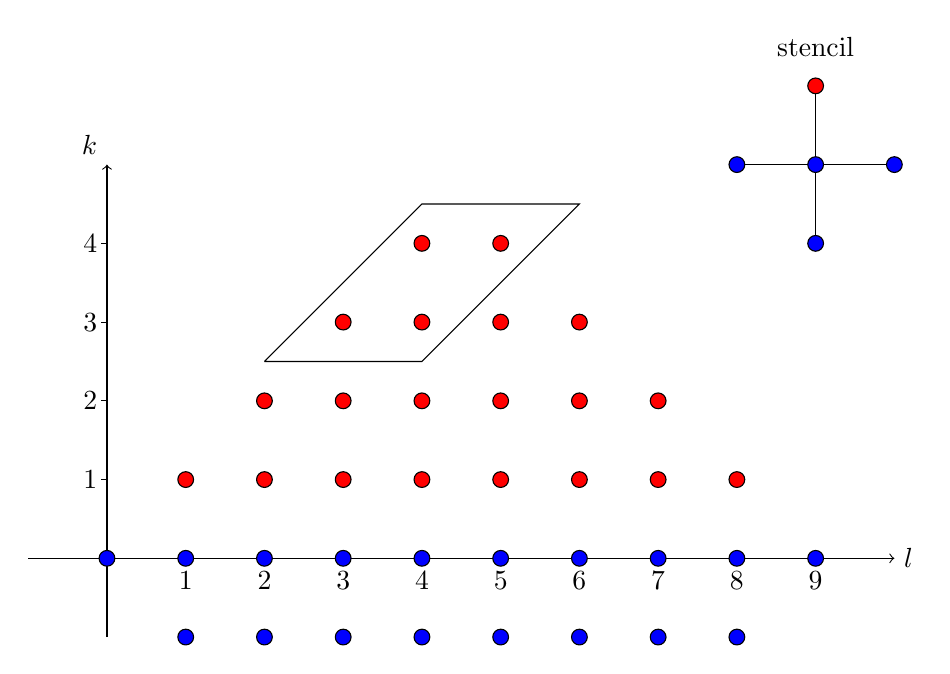
\begin{tikzpicture}[scale=1.0]
\draw[->] (0, -1) -- (0, 5);
\node[above left] at (0, 5) {$k$};
\draw[->] (-1, 0) -- (10, 0);
\node[right] at (10, 0) {$l$};
\foreach \x in {1, 2, ..., 8}
    \draw[fill=blue] (\x, -1) circle(0.10cm);
\foreach \x in {0, 1, ..., 9}
    \draw[fill=blue] (\x, 0) circle(0.10cm);
\foreach \x in {1, 2, ..., 8}
    \draw[fill=red] (\x, 1) circle(0.10cm);
\foreach \x in {2, 3, ..., 7}
    \draw[fill=red] (\x, 2) circle(0.10cm);
\foreach \x in {3, 4, 5, 6}
    \draw[fill=red] (\x, 3) circle(0.10cm);
\foreach \x in {4, 5}
    \draw[fill=red] (\x, 4) circle(0.10cm);
\foreach \y in {1, 2, 3, 4}
    {
    \draw[thin] (-0.075, \y) -- (0, \y);
    \node[left] at (0.0, \y) {$\y$};
    }
\foreach \x in {1, 2, 3, ..., 9}
    \node[below] at (\x, -0.04) {$\x$};
\draw[-] (9, 4) -- (9, 6);
\draw[-] (8, 5) -- (10, 5);
\draw[fill=blue] (8, 5) circle(0.10cm);
\draw[fill=blue] (9, 5) circle(0.10cm);
\draw[fill=blue] (10, 5) circle(0.10cm);
\draw[fill=blue] (9, 4) circle(0.10cm);
\draw[fill=red]  (9, 6) circle(0.10cm);
\node at (9, 6.5) {stencil};
\draw[-] (2.0, 2.5) -- (4.0, 4.5) -- (6.0, 4.5) 
      -- (4.0, 2.5) -- (2.0, 2.5);
\end{tikzpicture}
\end{center}
\caption{The dots correspond to the $\sigma_{lk}$ computed in the 
case~$n=5$.  The parallelogram indicates the $\sigma_{lk}$ used in 
the expressions for $\alpha_4$~and $\beta_4$.}
\end{figure}
\end{document}
